\documentclass[twoside]{article}\usepackage[]{graphicx}\usepackage[]{xcolor}
% maxwidth is the original width if it is less than linewidth
% otherwise use linewidth (to make sure the graphics do not exceed the margin)
\makeatletter
\def\maxwidth{ %
  \ifdim\Gin@nat@width>\linewidth
    \linewidth
  \else
    \Gin@nat@width
  \fi
}
\makeatother

\definecolor{fgcolor}{rgb}{0.345, 0.345, 0.345}
\newcommand{\hlnum}[1]{\textcolor[rgb]{0.686,0.059,0.569}{#1}}%
\newcommand{\hlsng}[1]{\textcolor[rgb]{0.192,0.494,0.8}{#1}}%
\newcommand{\hlcom}[1]{\textcolor[rgb]{0.678,0.584,0.686}{\textit{#1}}}%
\newcommand{\hlopt}[1]{\textcolor[rgb]{0,0,0}{#1}}%
\newcommand{\hldef}[1]{\textcolor[rgb]{0.345,0.345,0.345}{#1}}%
\newcommand{\hlkwa}[1]{\textcolor[rgb]{0.161,0.373,0.58}{\textbf{#1}}}%
\newcommand{\hlkwb}[1]{\textcolor[rgb]{0.69,0.353,0.396}{#1}}%
\newcommand{\hlkwc}[1]{\textcolor[rgb]{0.333,0.667,0.333}{#1}}%
\newcommand{\hlkwd}[1]{\textcolor[rgb]{0.737,0.353,0.396}{\textbf{#1}}}%
\let\hlipl\hlkwb

\usepackage{framed}
\makeatletter
\newenvironment{kframe}{%
 \def\at@end@of@kframe{}%
 \ifinner\ifhmode%
  \def\at@end@of@kframe{\end{minipage}}%
  \begin{minipage}{\columnwidth}%
 \fi\fi%
 \def\FrameCommand##1{\hskip\@totalleftmargin \hskip-\fboxsep
 \colorbox{shadecolor}{##1}\hskip-\fboxsep
     % There is no \\@totalrightmargin, so:
     \hskip-\linewidth \hskip-\@totalleftmargin \hskip\columnwidth}%
 \MakeFramed {\advance\hsize-\width
   \@totalleftmargin\z@ \linewidth\hsize
   \@setminipage}}%
 {\par\unskip\endMakeFramed%
 \at@end@of@kframe}
\makeatother

\definecolor{shadecolor}{rgb}{.97, .97, .97}
\definecolor{messagecolor}{rgb}{0, 0, 0}
\definecolor{warningcolor}{rgb}{1, 0, 1}
\definecolor{errorcolor}{rgb}{1, 0, 0}
\newenvironment{knitrout}{}{} % an empty environment to be redefined in TeX

\usepackage{alltt}
\usepackage[left=3cm, right=2cm, top=3cm, bottom=2cm]{geometry}
%\usepackage[brazil]{babel}
\usepackage[utf8]{inputenc}
\usepackage{amsmath, amssymb, amsfonts}
\usepackage{mathtools}
\usepackage{mathrsfs}
\usepackage{siunitx}
\usepackage{fancyhdr}
\usepackage{xcolor}
\usepackage{graphicx}
\usepackage{enumitem}
\usepackage{tikz}
\usepackage{mdframed} % Para criar caixas coloridas
\usepackage{float}
\usetikzlibrary{patterns,snakes}






% Define a cor principal do arquivo
\definecolor{mainColor}{HTML}{5b017d}

% Redefinir o comando \section para ter o mesmo tamanho que \subsection
\makeatletter
\renewcommand\section{\@startsection{section}{1}{\z@}%
                                     {-3.5ex \@plus -1ex \@minus -.2ex}%
                                     {2.3ex \@plus.2ex}%
                                     {\normalfont\large\bfseries}}
\makeatother


% Configuração do cabeçalho e rodapé
\pagestyle{fancy}
\fancyhf{} % Limpa os cabeçalhos e rodapés atuais

% Cabeçalho para páginas pares
\fancyhead[RE]{Igo da Costa Andrade}

% Cabeçalho para páginas ímpares
\fancyhead[LO]{
    Título do Livro (Autor1, Autor2)
}

\fancyhead[RO]{
    
}

% Número da página no rodapé (centrado)
\fancyfoot[C]{\thepage}

\newcommand{\capitulo}{1}

% Definir leftmargin=* para todos os ambientes enumerate
\setlist[enumerate,1]{leftmargin=*, resume, label=\textbf{\capitulo.\arabic*}}


\newcommand{\makecover}{
    \textcolor{mainColor}{\hrule}
    \vspace{0.25cm}
    \begin{minipage}[c]{12cm}
        \begin{center}
            \Large{
                Resolução de exercícios do Livro:\\
                \vspace{0.25cm}
                \textcolor{mainColor}{\textbf{Título do Livro (Autor1, Autor2)}}\\
                \vspace{0.7cm}
                \small{por}\\
                \vspace{0.2cm}
                \textbf{\large{Igo da Costa Andrade}}
            }
        \end{center}
        \vspace{0.25cm}
        \hrule
        \vspace{0.25cm}
        \textbf{Referência}
        
        \noindent AUTOR1, A.; AUTOR2, A. \textbf{Título do Livro}. Local: Editora, AAAA.
    \end{minipage}
    \begin{minipage}[c]{4cm}
    
        \begin{flushright}
            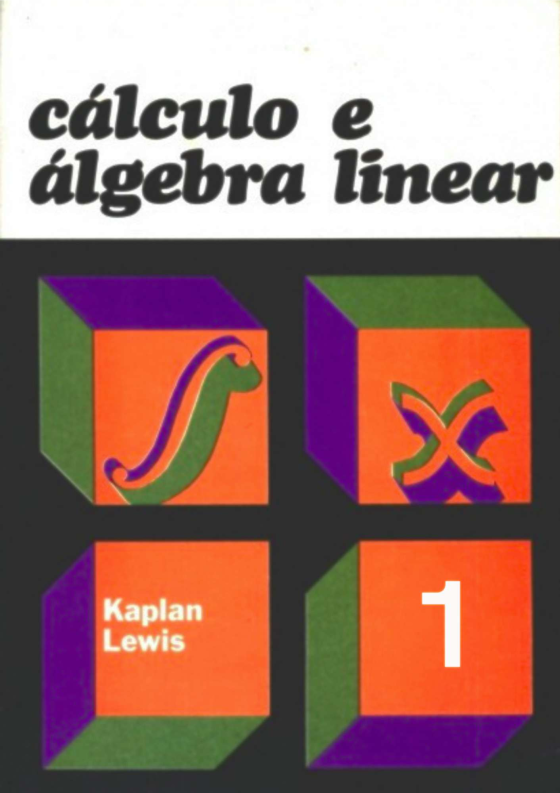
\includegraphics[width=0.8\linewidth]{img/capa.png}    
        \end{flushright}
        
    \end{minipage}
    \vspace{0.25cm}
    \textcolor{mainColor}{\hrule}
    
}

% Bold Vector
\newcommand{\vet}[1]{\mathbf{\hat{#1}}}

% Comando iniciar Solução
\newcommand{\iniSol}{
    \noindent\textcolor{mainColor}{\rule{0.3\textwidth}{0.4pt}}\\
    \noindent\textcolor{mainColor}{\textbf{Solução:}}\\
}

% Comando finalizar Solução
\newcommand{\fimSol}{
    %
    \hfill\fcolorbox{mainColor}{mainColor}

    
    \hfill\textcolor{mainColor}{\rule{0.3\textwidth}{0.4pt}}
}
\IfFileExists{upquote.sty}{\usepackage{upquote}}{}
\begin{document}
\thispagestyle{empty}

\makecover{}


\begin{center}
    \vspace{1cm}
    \textbf{\Large{\textcolor{mainColor}{Capítulo \capitulo:} Geometria vetorial em duas dimensões}}
    \vspace{1cm}

    \textbf{PROBLEMAS}
\end{center}

\begin{enumerate}
    \item Seja dado o triângulo $ABC$. Seja $\overrightarrow{AB} = \mathbf{u}$ e $\overrightarrow{AC} = \mathbf{v}$, e sejam os pontos $P$, $Q$ escolhidos de modo que $\overrightarrow{AP} = 3\mathbf{u}$, $\overrightarrow{AQ} = 2 \mathbf{v}$, como na Fig. 1.13. 


    \begin{figure}[H]
        \centering
        \text{Fig. 1.13}\\
        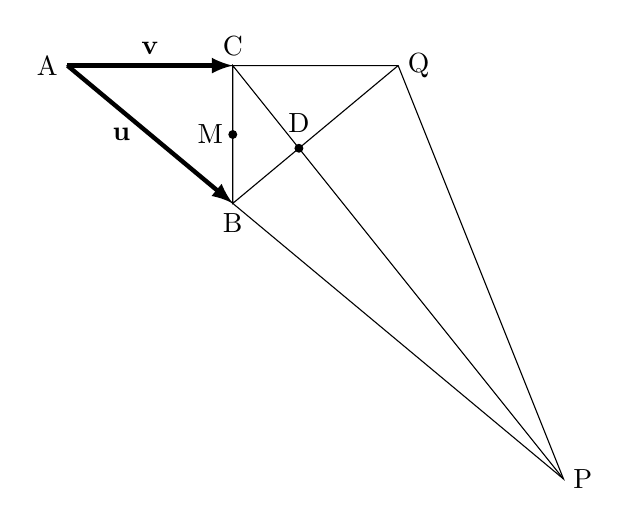
\begin{tikzpicture}[scale=0.7]
            \draw (0, 0) node[left] {A} -- (6, 0) node[right] {Q} -- (9, -7.5) node[right] {P} -- cycle; 
            \draw (9, -7.5) -- (3, 0) node[above] {C} -- (3, -2.5) node[below] {B} -- (6, 0);
            \filldraw (3, -1.25) circle (2pt) node[left] {M};
            \filldraw (4.2, -1.5) circle (2pt) node[above, yshift=2pt] {D};
            \draw[-latex, ultra thick] (0, 0)--(3, -2.5) node[midway, left, xshift=-3pt] {$\mathbf{u}$};
            \draw[-latex, ultra thick] (0, 0)--(3, 0) node[midway, above] {$\mathbf{v}$};
        \end{tikzpicture}      
    \end{figure}
    
    Exprima os seguintes vetores em função de $\mathbf{u}$ e $\mathbf{v}$: (a) $\overrightarrow{BC}$, (b) $\overrightarrow{PB}$, (c) $\overrightarrow{PQ}$, (d) $\overrightarrow{PC}$, (e) $\overrightarrow{BQ}$, (f) $\overrightarrow{AM}$, onde $M$ é o ponto médio de $\overrightarrow{BC}$, (g) $\overrightarrow{BD} + \overrightarrow{DC} + \overrightarrow{CQ}$.

    \iniSol
    
    \begin{enumerate}[label=(\alph*)]
        \item $\overrightarrow{BC}$
        \begin{align*}
            \overrightarrow{AC} = \overrightarrow{AB} + \overrightarrow{BC} &\Rightarrow \overrightarrow{BC} = \overrightarrow{AC} - \overrightarrow{AB}\\
            &\Rightarrow \overrightarrow{BC} = \mathbf{v} - \mathbf{u}
        \end{align*}
        
        \item $\overrightarrow{PB}$
        \begin{align*}
            \overrightarrow{AP} = \overrightarrow{AB} + \overrightarrow{BP} &\Rightarrow \overrightarrow{AP} = \overrightarrow{AB} - \overrightarrow{PB}\\
            &\Rightarrow \overrightarrow{PB} = \overrightarrow{AB} - \overrightarrow{AP}\\
            &\Rightarrow \overrightarrow{PB} = \mathbf{u} - 3\mathbf{u}\\
            &\Rightarrow \overrightarrow{PB} = -2 \mathbf{u}
        \end{align*}
        
        \item $\overrightarrow{PQ}$
        \begin{align*}
            \overrightarrow{AP} = \overrightarrow{AQ} + \overrightarrow{QP} & \Rightarrow \overrightarrow{AP} = \overrightarrow{AQ} - \overrightarrow{PQ}\\
            &\Rightarrow \overrightarrow{PQ} = \overrightarrow{AQ} - \overrightarrow{AP}\\
            &\Rightarrow \overrightarrow{PQ} = 2\mathbf{v} - 3\mathbf{u}
        \end{align*}
        
        \item $\overrightarrow{PC}$
        \begin{align*}
            \overrightarrow{AP} = \overrightarrow{AC} + \overrightarrow{CP} &\Rightarrow \overrightarrow{AP} = \overrightarrow{AC} - \overrightarrow{PC}\\
            &\Rightarrow \overrightarrow{PC} = \overrightarrow{AC} - \overrightarrow{AP}\\
            &\Rightarrow \overrightarrow{PC} = \mathbf{v} - 3 \mathbf{u}
        \end{align*}
        
        \item $\overrightarrow{BQ}$
        \begin{align*}
            \overrightarrow{AQ} = \overrightarrow{AB} + \overrightarrow{BQ} &\Rightarrow \overrightarrow{BQ} = \overrightarrow{AQ} - \overrightarrow{AB}\\
            &\Rightarrow \overrightarrow{BQ} = 2 \mathbf{v} - \mathbf{u}
        \end{align*}
        
        \item $\overrightarrow{AM}$, onde $M$ é o ponto médio de $\overrightarrow{BC}$
        Podemos escrever $\overrightarrow{AM}$ das seguintes formas:
        \begin{align*}
            \begin{cases}
                \overrightarrow{AM} = \overrightarrow{AB} + \overrightarrow{BM}, \text{ ou }\\
                \overrightarrow{AM} = \overrightarrow{AC} + \overrightarrow{CM}
            \end{cases}
        \end{align*}
        Como $M$ é o ponto médio de $\overrightarrow{BC}$, devemos ter $\overrightarrow{CM} = -\overrightarrow{BM}$. Assim, substituindo nas expressões acima, tem-se:
        \begin{align*}
            \begin{cases}
                \overrightarrow{AM} = \overrightarrow{AB} + \overrightarrow{BM}\\
                \overrightarrow{AM} = \overrightarrow{AC} - \overrightarrow{BM}
            \end{cases}
            &\Rightarrow 2 \overrightarrow{AM} = \overrightarrow{AB} + \overrightarrow{AC} \\&\Rightarrow \overrightarrow{AM} = \dfrac{\overrightarrow{AB} + \overrightarrow{AC}}{2}\\
            &\Rightarrow \overrightarrow{AM} = \dfrac{\mathbf{u} + \mathbf{v}}{2}
        \end{align*}
        
        \item $\overrightarrow{BD} + \overrightarrow{DC} + \overrightarrow{CQ}$
        \begin{align*}
            \overrightarrow{BD} + \overrightarrow{DC} + \overrightarrow{CQ} = \overrightarrow{BQ} = 2 \mathbf{v} - \mathbf{u}
        \end{align*}
    \end{enumerate}
    \fimSol

    \item Seja $ABC$ um triângulo, seja $M$ o ponto médio de $BC$ e $N$ o ponto médio do lado $AB$ (Fig. 1.14). Seja $R$ um ponto escolhido em $AM$ e $T$ em $CN$ tal que $|\overrightarrow{AR}|/|\overrightarrow{AM}| = 3/4$ e $|\overrightarrow{CT}|/|\overrightarrow{CN}| = 1/3$. Seja $\mathbf{u} = \overrightarrow{AB}$, $\mathbf{v} = \overrightarrow{AC}$. Exprima os seguintes vetores em função de $\mathbf{u}$ e $\mathbf{v}$: (a) $\overrightarrow{AB}$, (b) $\overrightarrow{BC}$
\end{enumerate}


\end{document}
